%Generally: improve formatting. Not pretty, but should be.

\documentclass[a4paper,twoside]{article}

\usepackage{a4wide}
\usepackage[utf8]{inputenc}
\usepackage[T1]{fontenc}
% Better font
\usepackage{lmodern}
% Better font rendering
\usepackage{microtype}
% Packages for pictures:
\usepackage{graphicx}
\usepackage{float}
% Package for urls:
\usepackage{url}
\usepackage{hyperref}
%Take care of header:
\usepackage{fancyhdr}
%Define bib style:
\bibliographystyle{alpha}

%Prepare header & footer:
\pagestyle{fancy}
\fancyhead{}
\fancyfoot{}
\renewcommand{\sectionmark}[1]{\markright{\MakeUppercase \thesection.\ #1}}
\fancyhead[RO] {\rightmark}
\fancyhead[LE] {\author{Tamino Hartmann}}
\fancyfoot[RO, LE] {\thepage}

%Alternative paragraph style
\setlength{\parindent}{0.0in}
\setlength{\parskip}{0.1in}

\begin{document}

\title{Implementation of a Java Framework for Marker Based Detection in Augmented Reality \\ {\large Proposal}}
\author{Tamino Hartmann}
\date{\today}

\maketitle
\thispagestyle{empty}

\begin{abstract}
This paper represents the proposal of the bachelor thesis for Tamino Hartmann.
The goal is the development of an Android framework written in Java to allow the detection and usage of printed markers in augmented reality via a device's camera.
To prove the concept, the framework will be developed right into a first application that will implement it.
\end{abstract}

%Leave an empty page:
\newpage
\mbox{}

%And now get to the table of contents:
\newpage

\tableofcontents

\newpage

\section*{TODO}

\begin{itemize}
	\item I need a catchy name for the framework and for the app that will come from it (simply that they can be referenced easily and quickly).
	\item Improve on the title page. Should be consistent until the end of my work.
	\item Improve the introduction. Especially the URL-jungle. :P
\end{itemize}

\section{Introduction}

This paper represents the proposal developed by Tamino Hartmann as his bachelor thesis at the Faculty of Engineering and Computer Science\footnote{See: \url{http://www.uni-ulm.de/en/in/faculty-of-engineering-and-computer-science.html}.} at the Institute of Databases and Information Systems\footnote{See: \url{http://www.uni-ulm.de/en/in/dbis.html}.} at the University of Ulm\footnote{See: \url{http://www.uni-ulm.de/en/homepage.html}.}.
The supervisor is Marc Schickler\footnote{See: \url{http://www.uni-ulm.de/en/in/dbis/team/marc-schickler.html}.} and the examiner is Professor Doctor Manfred Reichert\footnote{See: \url{http://www.uni-ulm.de/en/in/iui-dbis/staff/manfred-reichert.html}.}.
The work was commissioned as a bachelor thesis to create a framework for fast and easy integration of marker-based tracking for future projects.

The goal of the framework will be reached by programming an application that uses it.
The framework will be initially based on the Android\footnote{See: \url{http://www.android.com/}.} port\cite{opencvandroid} of OpenCV\cite{opencv}, implemented as a Java package.
Ideally, the final version will run independent of the OpenCV module beneath it, although we do not guarantee that functionality at the moment for the final version.
Should the OpenCV library be freely exchangeable, the framework will also be usable beyond Android.

To develop and test the framework right from the start, we will develop an Android application (henceforth app) that implements it.
The app will allow for the real-time viewing of virtual objects on top of a marker.
By moving the device, the object can be viewed from different perspectives.
This shall prove the capability and initial concept of the framework and also serve as a starting point for any future work.

This paper consists of all the work done before any actual implementation is done.
We will look at the basic requirements of the framework and app.
Basic necessities will be listed and reviewed.
We'll also present mockups of the final app and a proposal for the structure of the framework.
However, the results may vary at the end for both the look of the app and the structure of the framework, so we claim no responsibility for their correctness as of now.
The final state will be compared to the proposed state in a second paper, in which we will look back at the development and summarize the important aspects.

Apart from the programmatic development of the framework, the app, and the final review of our work, we will also deliver at least basic documentation for the framework and app.
For the framework this will at least include a Javadoc\footnote{See: \url{http://en.wikipedia.org/wiki/Javadoc}.} file for the complete code and a basic tutorial for usage.
For the app, we expect little documentation to be required for the usage.
Therefore, we propose implementing a basic helping function within the app either as contextual tips or manual pages accessible from within the app.
The code for the app will also include a Javadoc file.

\section{App Design}

Within these sections we will discuss the graphical interface of the app and its control flow.

\subsection{Control Flow}

TODO: Flowchart etc.

\subsection{Mockups}

Upon starting the app on a capable device, the app presents itself as shown in Figure \ref{fig:start_mockup}.
This is effectively the start screen from where all the interaction takes place.
The green light in the top left shows that the app is detecting the marker with a high confidence, meaning that there are no large uncertainties.
If the marker is too warped or partially covered, the light switches to red.
If the app can still detect the marker but is having difficulties, the light switches to orange.
This mechanism is meant to offer fast and accurate feedback to the detection capability.
Another method of direct feedback is the already displayed axis-object.
This is meant to offer fast feedback to the orientation and scaling of the coordinate space to the user before a custom object is displayed.
The visibility of the axis-object can be toggled in the settings.

The menu button on the status bar at the bottom of the screen opens up a menu as seen in Figure ???.
From here the user can control the overlays they wish displayed over the camera view and control what is rendered into the picture.

\begin{figure}
	\centering
	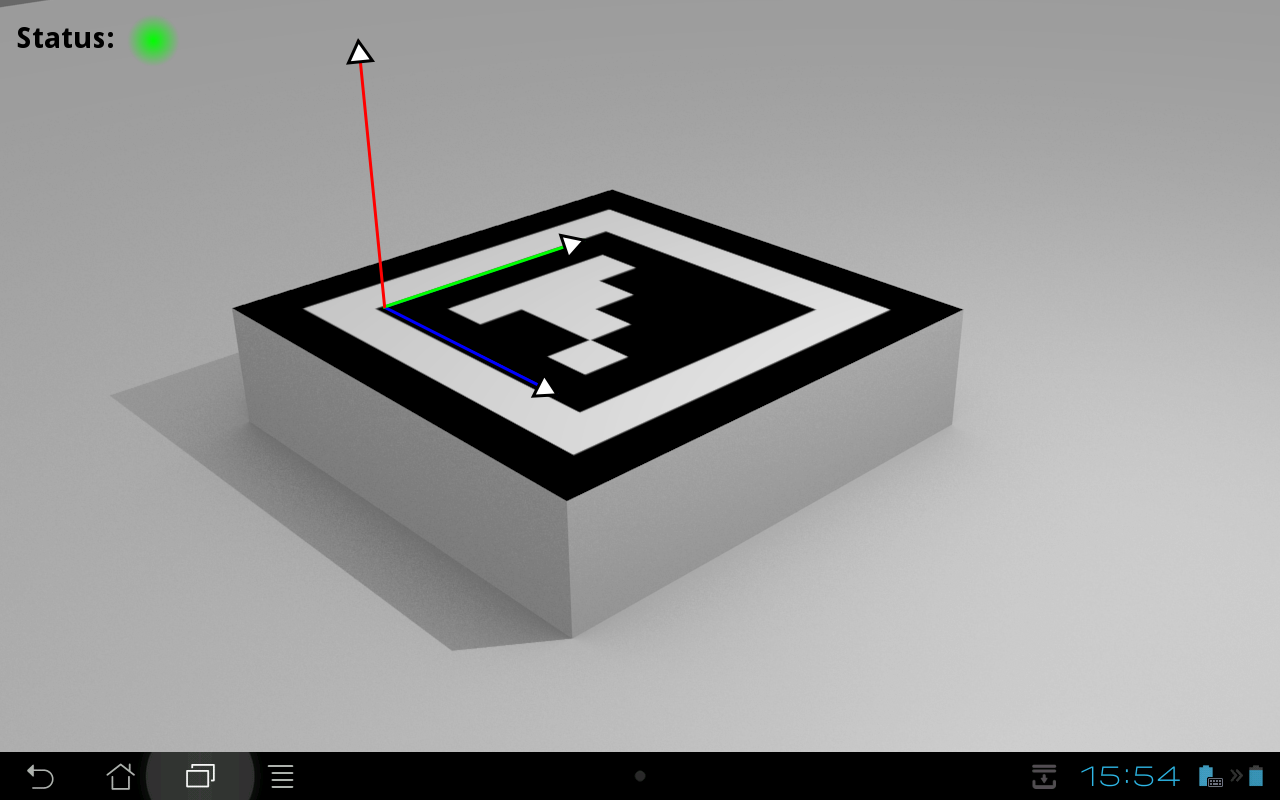
\includegraphics[width=15cm]{images/start_mockup.png}
	\caption[Start screen mockup.]{Mockup of how the start screen of the final app might look. Note the menu button on the bottom, the rendered axes, and the green status light signifying that the marker is being read with a high confidence.}
	\label{fig:start_mockup}
\end{figure}

\section{Framework API}

In this section, we take a close look at the proposed structure and capabilities of the framework's API.
The final implementation will however deviate with a high probability.

\section{Conclusion}

TODO...

\newpage

\listoffigures
%\listoftables
\bibliography{doc}

\end{document}